\documentclass[a4paper, 11pt, twoside]{article}
\usepackage{amssymb}
\usepackage{amsmath}
\usepackage{bm}
\usepackage{graphicx}
\begin{document}
\title{STAT6038 Week 8 Lecture Notes}
\author{xarskii}
\date{2017-04-26}

\maketitle

\section{Wednesday Lecture}
\subsection{Estimation and Prediction using Multiple (MR) Regression models}
Estimate of $Y$ given new values of the $X$ variables

\[
\begin{split}
	\hat{Y}|\bm{x_0}&=\hat{\beta_0}+\hat{\beta_1}x_{01}+\hat{\beta_2}x_{02}+\cdots +\hat{\beta_k}x_{0k}\\
	&=\bm{x}^T_0\bm{\hat{\beta}}
\end{split}
\]

where $\bm{x_0}=\begin{pmatrix}1\\x_{01}\\x_{02}\\x_{03}\\\vdots\\x_{0k}\end{pmatrix}, \bm{\hat{\beta}}=\begin{pmatrix}\hat{\beta_0}\\\hat{\beta_1}\\\vdots\\\hat{\beta_k}\end{pmatrix}.$


\[
\begin{split}
	\text{Var}(\hat{Y}|x_0)&=\text{Var}(\bm{x_0}^T\bm{\hat{\beta}})\\
	&=\bm{x_0}^T\text{Var}(\bm{\hat{\beta}})(\bm{x_0}^T)^T\\
	&=\sigma^2\bm{x_0}^T(X^TX)^{-1}\bm{x_0}
\end{split}
\]

So, a $100(1-\alpha)\%)$ confidence interval for $E[Y|\bm{x_0}]$ is $\hat{Y}|\bm{x_0}\pm t_{n-p}(1-\frac{\alpha}{2})s\sqrt{\bm{x_0}^T(X^TX)^{-1}\bm{x_0}}$ (of SLR $\hat{Y}|x^{*}\pm t_{n-2}(1-\frac{\alpha}{2})s\sqrt{\frac{(x^*-\bar{x})^2}{\text{SS}_x}}$)

And, a $100(1-\alpha)\%$ prediction interval for $Y|\bm{x_0}$ is $\hat{Y}|\bm{x_0}\pm t_{n-p}(1-\frac{\alpha}{2})s\sqrt{1+\bm{x_0}^T(X^TX)^{-1}\bm{x_0}}$

$\rightarrow$ again, we leave the implementation of these formulae to R and use the \texttt{predict()} function.

\subsection{Problem of Multiple Comparisons}

Forming a 95\% interval estimate (prediction or confidence interval) is directly related to a two-sided hypothesis test.

\begin{itemize}
	\item both types of inference are forms of comparisons.\\
	In forming 3 intervals, we have made 3 comparisons, all at the 95\% confidence level.\\
	\textbf{Is our overall confidence 95\%?}\\
	No, with $m$ comparisons, it is closer to
	\[
	\begin{split}
		P(\text{all ``tests'' accepted)})&=1-P(\text{at least one test is rejected})\\
		&\geq 1-\sum^m_{i=1}P(\text{each test is rejected})\ \ \ \text{(relies on Boole's inequality)}\\
		&=1-m\alpha
	\end{split}
	\]
	See Faraway text, pg 87.
\end{itemize}

In this instance, $m=3$ comparisons, each at $\alpha=0.05$.

So, our overall confidence is $\simeq 1-3(0.05)=0.85$ i.e. 85\%.

If we know in advance (a priori) that we are going to make $m=3$ comparisons, we could solve $1-m\alpha=0.95\implies m\alpha=1-0.095\implies m\alpha=0.05\implies \alpha=\frac{0.05}{m}=0.0167$ i.e. do the 3 ``tests'', all at the $\alpha=0.0167$ level of significance or $(1-\alpha) 100\% = 0.9833\times 100\%$, i.e. 98.3\% confidence  intervals.

This $(1-\alpha/m)$ correction is called  the \textit{Bonferroni} (1936) correction. 

\section{Thursday Lecture}

\texttt{predict(..., interval="prediction")} vs. \texttt{predict(..., interval="confidence")}

\subsection{Residual Diagnostics}

Raw residual for hte $i^{\text{th}}$ observation

\[e_i = Y_i - \hat{Y_i}\]

$\rightarrow$ these are estimates of the errors $\epsilon_i$ i.e. $e_i=\hat{\epsilon_i}$

Note the assumptions about the errors, $\text{Var}(\epsilon)=\sigma^2I$, but (see earlier) $\text{Var}(e)=\sigma^2(I-H)$ where $H$ is the hat matrix.

So, the \textbf{standardized} (internally Studentised) residuals for the $i^{\text{th}}$ observation are:

\[r_i=\frac{e_i-0}{\sqrt{\sigma^2(1-h_{ii}}}\simeq\frac{e_i}{\sqrt{\text{MS}_{\text{error}}}(1-h_{ii})}\]

where $h_{ii}$ is the hat value (leverage) of the $i^{\text{th}}$ observation, and we use $\hat{\sigma}^2=s^2=\text{MS}_{\text{error}}$ to estimate the unknown $\sigma^2$.

So

\[r_i=\frac{e_i}{s\sqrt{1-h_{ii}}}\]

As $\sigma^2$ is estimated these are approximated distributed as a Student's t distribution.

\subsection{Residual Plots (Ian's preferred plots)}

\begin{enumerate}
	\item Main residual plot\\
	Standardized (internally Studentized) residuals ($r_i$) against the fitted values ($\hat{Y_i}$)\\
	$\rightarrow$ we should check this for every model we fit.\\
	$\rightarrow$ why? checks the key assumptions of independence and constant variance.
	\item Normal quantile plot (of the standardized residuals)\\
	Default \texttt{plot(model, which=2)} works fine\\
	$\rightarrow$ only bother checking once \textbf{plot 1} is okay\\
	$\rightarrow$ checks assumption of normality\\
	$\rightarrow$ could add $45^{\circ}$ line for comparison (\texttt{abline(0, 1, lty=2)})
	\item Outlier/Influence plot\\
	My preference is a bar plot of Cook's distances.\\
	\texttt{plot(model, which=4)}\\
	$\rightarrow$ only really need if there is some indication that outliers and/or influential points might be a problem on \textbf{plots 1 and/or 2}.\\
	$\rightarrow$ can further investigate - check leverage values (bar plot)\\
	$\rightarrow$ could also use \texttt{plot(model, which=5)} (but ignore the arbitrary cut-offs for Cook's distance)\\
	$\rightarrow$ also, we could perform a test ...
\end{enumerate}

\section{Friday Lecture}

\subsection{Deletion Residual}
Also called \textbf{PRESS} residuals, ``Prediction Sum of Squares''.

\[e_{i, -i}=Y_i-\hat{Y}_{i, -i}\]

where $\hat{Y}_{i, -i}$ is the fitted value for the $i^{\text{th}}$ observation based on a model which has been fitted to the data with the $i^{\text{th}}$ observation deleted (or excluded).

Surely this involves fitting a model (so we can calculate $e_{i,-i}$ for each $i=1,2,\dots, n$)?

No, as it can be shown that

\[e_{i,-i}=\frac{e_i}{1-h_{ii}}\]

and these deletion residuals have $\text{Var}(e_{i,-i})=\frac{\sigma^2}{1-h_{ii}}$.

So, if we standardize the deletion residuals

\[\frac{e_{i,-i}-0}{\sqrt{\sigma^2/(1-h_{ii}}}\simeq\frac{e_{i,-i}}{\sqrt{s^2/(1-h_{ii}}}=\frac{e_i}{(1-h_{ii})s\sqrt{1/(1-h_{ii})}}=\frac{e_i}{s\sqrt{1-h_{ii}}}=r_i\]

Same standardized (internally Studentized) residuals as before!

But the internally Studentized residuals

\[r_i=\frac{e_i}{s\sqrt{1-h_{ii}}}\]

are called ``internally''  Studentized as the estimate of $\sigma^2$ used is based on a model which uses all data (including the current or $i^{\text{th}}$ observation).

Again, we can derive as estimate of $\sigma^2$ that excludes the current observation without to fit the entire model to a new reduced data set -- it turns out

\[S_{-i}=\sqrt{\frac{(n-p)s^2-e_i/(1-h_{ii})}{n-p-1}}\]

Note the new degrees of freedom used here (based on $1$ less observation) as $n-p-1$.

This gives an alternative type of standardized residuals: \textbf{the externally Studentized residuals}.

\[t_i=\frac{e_i}{s_{-i}\sqrt{1-h_{ii}}}=\frac{e_{i,-i}}{s_{-i}/\sqrt{1-h_{ii}}}\]

this version clearly shows that both the numerator (the deletion residual) and the denominator (a fixed function of the deletion $s$ estimate) come from a model with the $i^{\text{th}}$ observation excluded, hence the name ``externally`` Studentized residuals.\\

Back to the Pine example,

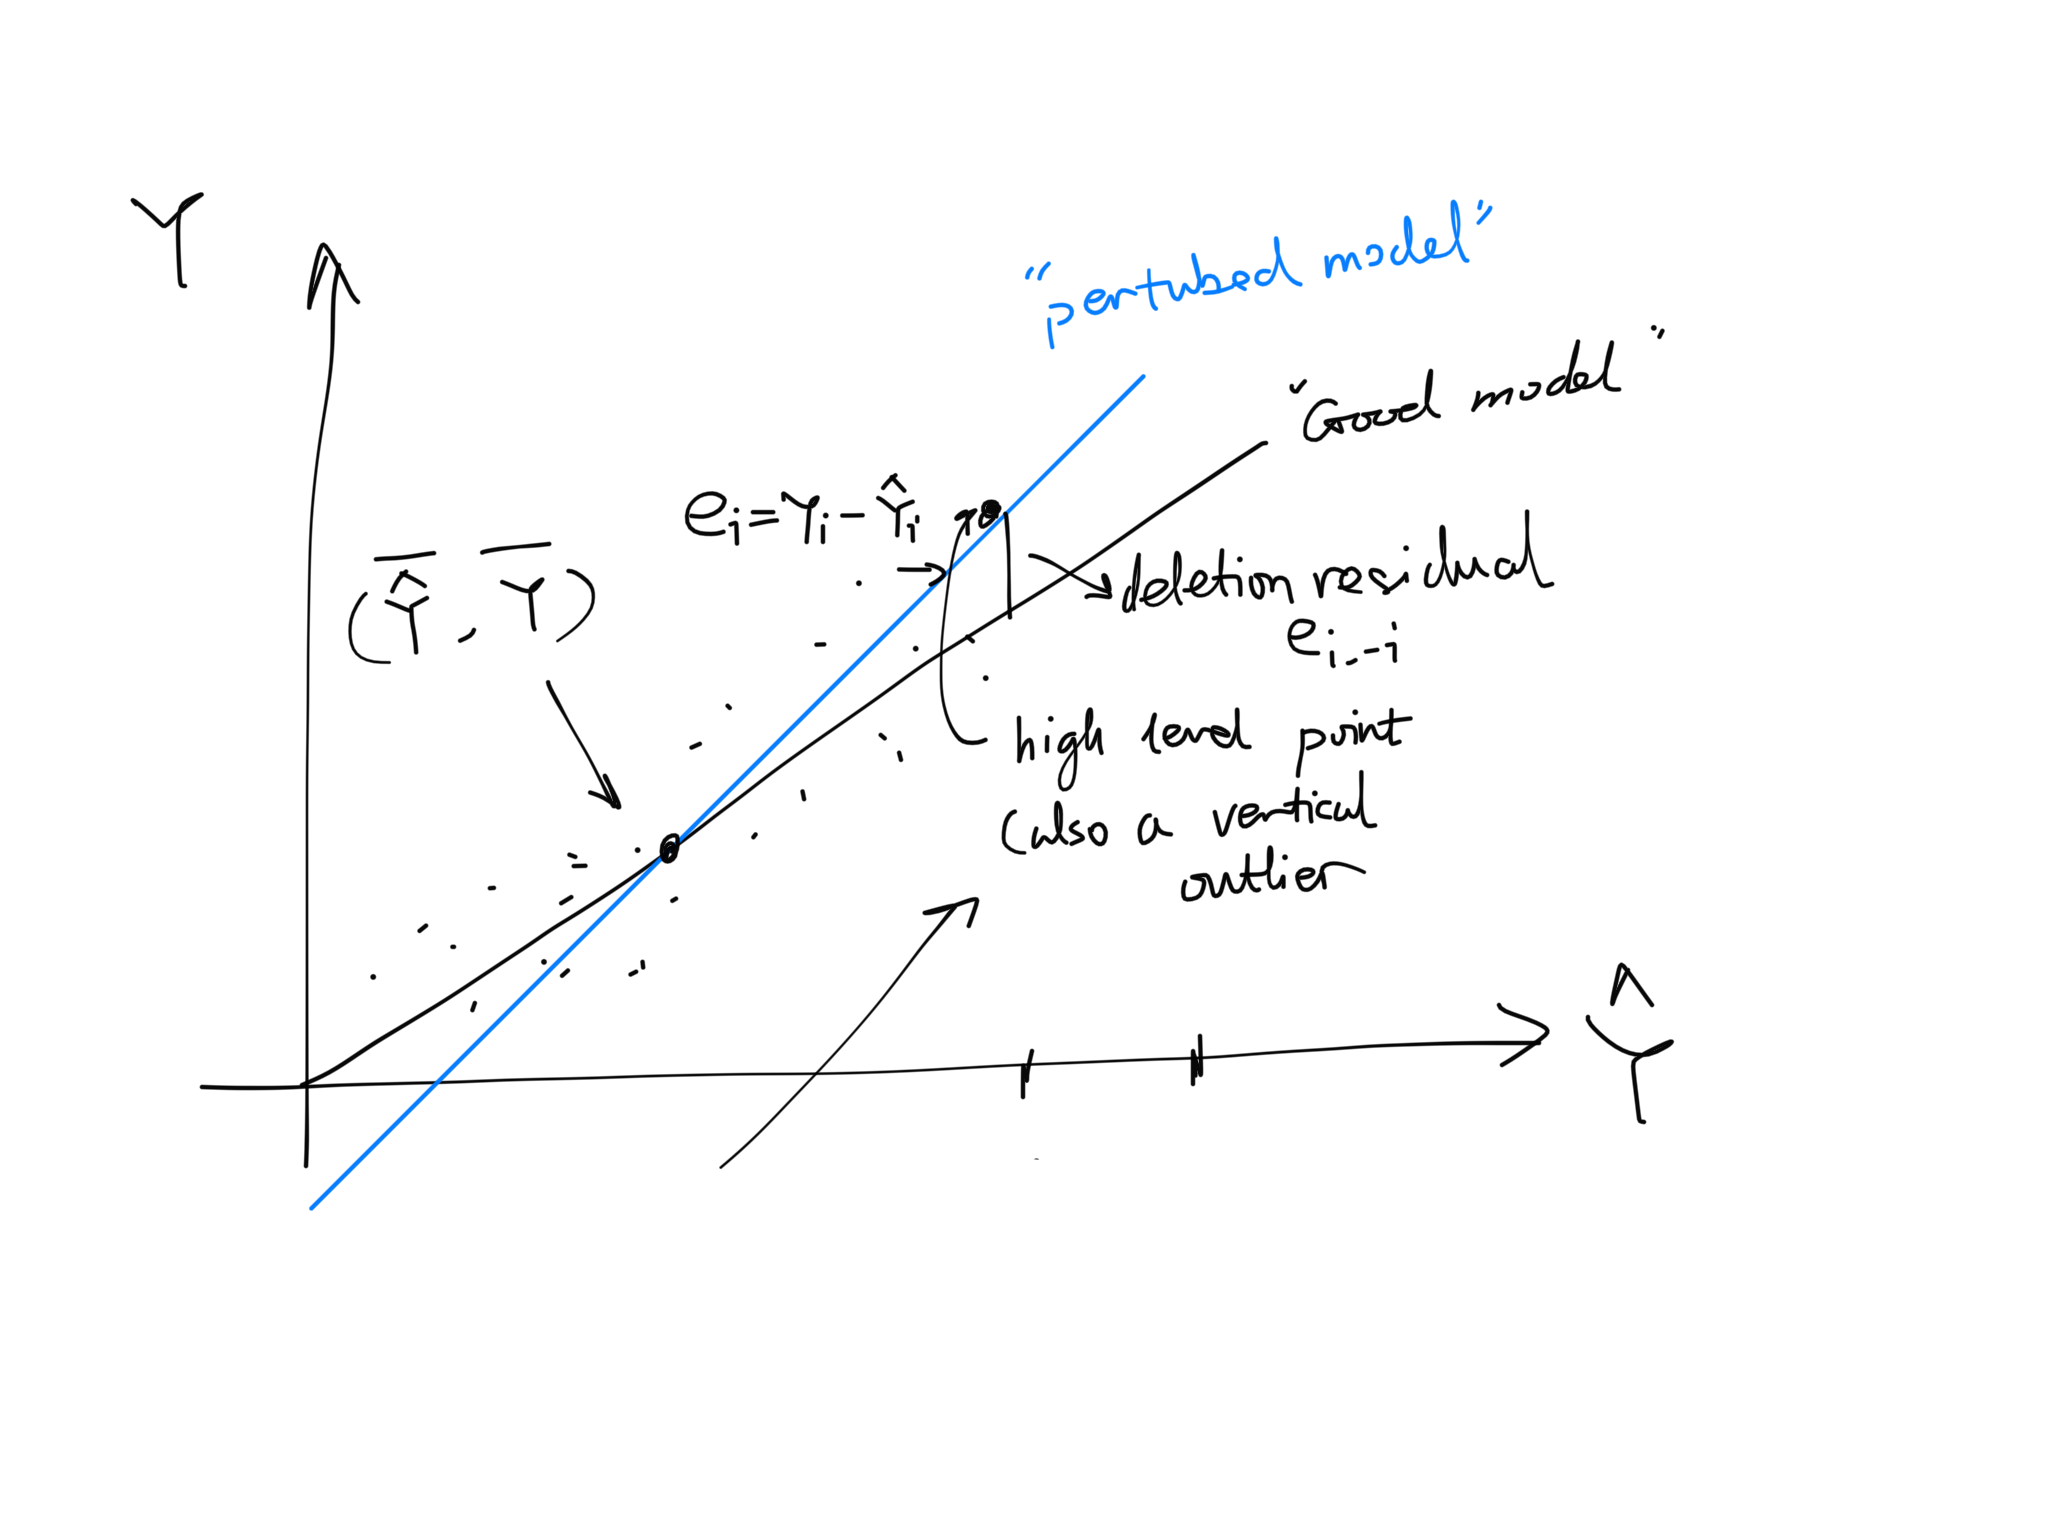
\includegraphics[width=\textwidth]{pine}

Example observation 20 in the full model (\texttt{pine.lm}) for the pine data.

indicator variable $I_i=\begin{cases}
	0\ \text{if}\ i=1,2,\dots, 19\\
	1\ \text{if}\ i=20
\end{cases}$

fitted model

\[\hat{Y}=\hat{\beta_0}+\hat{\beta_1}x_1+\hat{\beta_2}x_2+\hat{\beta_3}x_3+\hat{\beta_4}I_{20}\]

if $I_{20}=0\implies \hat{Y}=\hat{\beta_0}+\hat{\beta_1}x_1+\hat{\beta_2}x_2+\hat{\beta_3}x_3$

if $I_{20}=1\implies \hat{Y}=(\hat{\beta_0}+\hat{\beta_4})+\hat{\beta_1}x_1+\hat{\beta_2}x_2+\hat{\beta_3}x_3$

...

another plot\\

``Observation 20 failed the full model but passed the reduced model.''

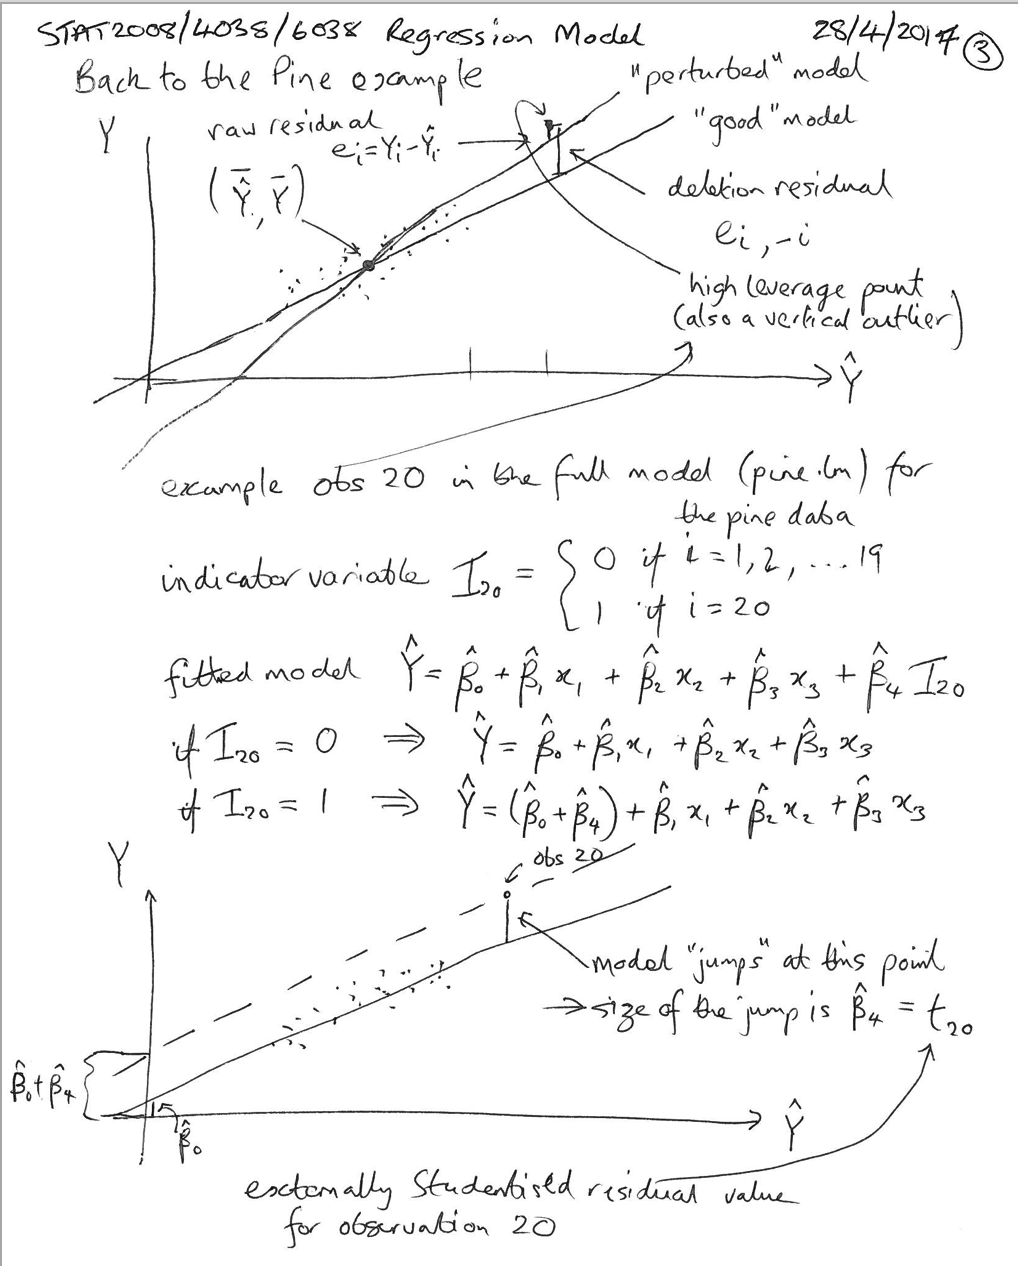
\includegraphics[width=\textwidth]{pine2.png}



\end{document}